\section{$B\bar{B}$ Oszillations \cite{bb}}
For a long time the measurement of $B$ oscillations was considered impossible. In 1986/87 measurements of the decay width of $B$ mesons showed that it was smaller than expected and thus oscillations could be observed. In 1987 they were finally discovered by the ARGUS experiment at DESY.
\subsection{Theoretical principles}
The 2-dimensional Cabibbo matrix was the first attempt to describe the difference between mass and weak eigenstates in the quark sector. The CKM matrix was an expansion to this theory by considering at least three generations of quarks. The CKM matrix provides four independent parameters, three mixing angles and one complex phase. This phase is the origin of $CP$ violation in weak interactions. Another form of representation for the CKM matrix is the Wolfenstein parameterization. The hierachy of the different entries is expressed by orders of $\lambda = \sin \vartheta_{12} \approx 0.22$.\\
The time evolution of unmixing mesons is given by the exponential decay law. For mixing mesons the Schrödinger equation is extended to a two-dimensional equation system. The mass eigenstates $B_{L}$ and $B_{H}$ can be extracted by diagonalizing the system. The weak eigenstates $B^0$ and $\bar{B}^0$ are linear combinations of these mass eigenstates. Both mass eigenstates have different masses and independent decay widths. For $B$ mesons it is possible to use the approximation of nearly equal decay widths for both mass states.
Therefore the weak eigenstates can be written as follows:
\begin{align*}
	\ket{B^{0}(t)} &= \frac{1}{2p}(\ket{B_{L}(t)} + \ket{B_{H}(t)}) &= \frac{e^{-\Gamma t/2}}{2}[(e^{-im_Lt}+e^{-im_Ht})\ket{B^0} + \frac{q}{p}(e^{-im_Lt}-e^{-im_Ht})\ket{\bar{B}^0}]\\
	\ket{\bar{B}^0(t)} &= \frac{1}{2q}(\ket{B_L(t)} - \ket{B_H(t)}) &= \frac{e^{-\Gamma t/2}}{2}[(e^{-im_Lt}+e^{-im_Ht})\ket{\bar{B}^0} + \frac{p}{q}(e^{-im_Lt}-e^{-im_Ht})\ket{B^0}]
\end{align*}
Therefore the oscillation probabilites are given by:
\begin{align*}
	P(B^0\rightarrow B^0 [\bar{B}^0]) = |\langle [\bar{B}^0] B^0 | B^0 \rangle|^2 = [\left| \frac{q}{p} \right|^2 ] \frac{e^{-\Gamma t}}{2} (1 \pm \cos (\Delta m t))
\end{align*}
This leads to the conclusion that the $CP$ asymmetry only depends on the mass difference of both states and the flight-time:
\begin{align*}
	A_{CP} = \frac{P(B^0\rightarrow B^0) - P(B^0\rightarrow \bar{B}^0)}{P(B^0\rightarrow B^0) + P(B^0\rightarrow \bar{B}^0)} = \cos(\Delta m t)
\end{align*}
The most common measurements of $B$ mesons are performed with $B_d^0\bar{B}_d^0$ and $B_s^0\bar{B}_s^0$. This leads to $\Delta m_d \sim m_t^2|V_{tb}V_{td}|^2 \sim m_t^2 \mathcal{O}(\lambda^6)$ and $\Delta m_s \sim m_t^2|V_{tb}V_{ts}|^2 \sim m_t^2 \mathcal{O}(\lambda^4)$.
Since $\Delta m_s \sim \frac{1}{\lambda^2} \Delta m_d$ the $B_s^0$ meson oscillates much faster than $B_d^0$.
\subsection{ARGUS}
The basic principle for the measurement of $B\bar{B}$ oscillation is to produce the $\Upsilon(4s)$ resonances at $e^+e^-$ colliders that decay approximately \SI{50}{\percent} of the time into $B\bar{B}$ pairs. Afterwards all events containing a $B$ meson pair need to be reconstructed to determine the decay ratio $r = \frac{N(B^0B^0)+ N(\bar{B}^0\bar{B}^0)}{N(B^0\bar{B}^0)}$. If $r>0$ $B\bar{B}$ oscillations exist. The considered decay of $B$ mesons does involve $D$ mesons, that then decay into $K$ and $\pi$ mesons.\\
The collision point of the ARGUS experiment was surrounded by a vertex chamber, followed by drift chambers and time of flight counters in front of shower counters. These were followed by solenoid coils and iron yokes in front of the muon chambers. In the direction of the beam pipe the vertex chamber was followed by compensation coils in front of mini beta quadrupoles. \\
The mini beta quadrupoles were placed inside the detector to improve the luminosity. The compensation coils ensured that the magnetic fields of the quadrupoles did not interfere with the solenoid. If a charged particle traveled through the drift chamber, it ionized the gas along its flight path. Together with the solenoid this provided a good momentum resolution. The time of flight counters were made out of scintillation counters. By measuring the flight time, they provided a possibility to determine the velocity of charged particles. Together with the momenta, it was possible to itentify particles over their rest mass.
\subsection{Performed Measurement}
\begin{wrapfigure}{l}{0.35\textwidth}
    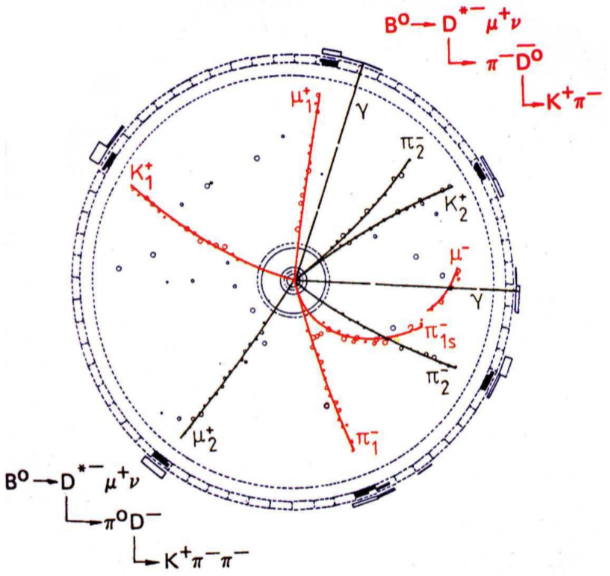
\includegraphics[width=0.33\textwidth]{graphics/BBbar.png}
    \caption{ARGUS event display of a $B^0B^0$ event.\cite{bb}}
		\label{fig:bb}
  \end{wrapfigure}
  \FloatBarrier
They used three different methods to reconstruct the events. The first method is a full event reconstruction, which has the smallest background. But the statistics are too small to determine $r$.  The second method is to reconstruct semi leptonic decays, which leads to higher statistics, but misidentification of leptons and therefore of $B$ mesons. Figure \ref{fig:bb} shows a possible event display. Different backgrounds are e.g. continuum dilepton sources or lepton hadron misidentification. They get supressed with momentum and angle cuts as well as using information from invariant masses to reject background events from resonance decays. The background analysis was also performed with data from well known decays to improve it.
\begin{align*}
	r &= \frac{[N(l^+l^+) + N(l^-l^-)(1+\lambda)]}{N(l^+l^-)-[N(l^+l^+)+N(l^-l^-)]\lambda} = 0.22 \pm 0.09 \pm 0.04 \\
	\text{with} \,\,  \lambda &= \frac{f^+}{f^0}\left( \frac{\text{Br}^+}{\text{Br}^0} \right)^2 = 1.2
\end{align*}
The third method is a compromise between the first two, which reduces the background. This method fully reconstructs one $B$ meson and the other one is tagged with a semi leptonic decay. The uncertainties are bigger since the statistics are smaller.
\begin{align*}
	r = \frac{N(B^0l^+)+N(\bar{B}^0l^-)}{N(B^0l^-)+N(\bar{B}^0l^+)} = 0.20 \pm 0.12
\end{align*}
The combined result is $r=0.21\pm0.08$ and is a clear evidence for $B\bar{B}$ oscillations.\\
The ratio is also proportional to $\Delta m$, which allows to set a lower limit to the top quark mass of $m_t \geq \SI{50}{\giga\electronvolt}$.\\

The LHCb collaboration performed high precision measurements of $B_d^0$ and $B_s^0$ meson oscillations.
They determined the mass differences to be:
\begin{align*}
	\Delta m_d &= 0.5156 \pm 0.0051 (\text{stat.}) \pm 0.0033 (\text{syst.})/ \si{\pico\second}\\
	\Delta m_s &= 17.768 \pm 0.023 (\text{stat.}) \pm 0.006 (\text{syst.})/ \si{\pico\second}
\end{align*}
